\documentclass[a4paper,10.5pt]{report}

\usepackage[toc]{appendix}
\renewcommand{\appendixname}{Annexos}
\renewcommand{\appendixtocname}{Annexos}
\renewcommand{\appendixpagename}{Annexos}
\usepackage[catalan]{babel}
\usepackage{booktabs}
\usepackage{listings}
\lstdefinestyle{mystyle}{
	language=Python,                 % Lenguaje del código
	frame=single,                    % Marco alrededor del código
	basicstyle=\ttfamily\footnotesize, % Fuente del código
	keywordstyle=\color{blue},       % Color para palabras clave (def, if, else...)
	commentstyle=\color{gray},       % Color para comentarios
	stringstyle=\color{teal},        % Color para strings
	numbers=left,                    % Numeración de líneas
	numberstyle=\tiny\color{gray},   % Estilo de los números de línea
	stepnumber=1,                     % Cada cuántas líneas numerar
	showspaces=false,                 % No mostrar espacios en blanco
	showstringspaces=false,            % No mostrar espacios en strings
	breaklines=true,                   % Romper líneas largas automáticamente
	tabsize=4,                         % Tamaño de tabulación
	captionpos=b,                      % Posición de la caption (arriba o abajo)
	morekeywords={self, as, in},       % Palabras clave adicionales
}
\lstset{style=mystyle} % Aplicar este estilo a todos los listados
\usepackage{tcolorbox}
\usepackage{parskip}
\usepackage{multirow}
\usepackage{graphicx}
\usepackage{booktabs}
\usepackage{caption}
\captionsetup{labelfont=bf}
\usepackage{hyperref}
\usepackage[arrowdel]{physics}
\usepackage[left=1.95cm, right=1.95cm, top=20mm, bottom=20mm]{geometry} 
\usepackage{fancyhdr}
\usepackage{braket}
\usepackage{amsmath, amssymb, amsfonts}
\usepackage{subcaption}
\usepackage{cancel}
\usepackage{float}
\usepackage{titling}
\usepackage{etoolbox}

%Definim el següent entorn per tal de poder posar abstracts a cada capítol.
\newenvironment{chapterabstract}{
	\begin{center}
		\bfseries Abstract
	\end{center}
	\quotation
}{\endquotation}

\usepackage{titlesec}
\usepackage{tikz}


\titleformat{\chapter}[display]{\normalfont\huge\bfseries}{Pràctica \thechapter}{0pt}{\vspace{0.2cm}\huge\bfseries\raggedright}

\title{\textbf{\huge{Informes de Pràctiques. \\ \vspace{0.2cm} Laboratori d'Electromagnetisme}}}
\author{Grup A1}
\date{\today}

\begin{document}
	
\begin{titlepage}
	\centering
	{\LARGE Laboratori d'Electromagnetisme \par}
	\vspace{2cm}
	{\Huge \textbf{Informes de Pràctiques} \par}
	\vspace{3cm}
	{\Large Grup A1 \par}
	\vspace{0.5cm}
	{\Large 1549086: Bujones Umbert, Jun Shan\\1669619: Rama Ariza, Raul\\  1672980: González Barea, Eric\\1644841: Vilarrúbias Morral, Natàlia \par}
	\vspace{2cm}
	{\Large Març $-$ Maig 2025 \par}
	\vspace{2cm}
	
	\begin{figure}[h]
		\centering
		
\includegraphics[width=0.3\linewidth]{screenshot001}
		\label{fig:screenshot001}
	\end{figure}
\end{titlepage}

\tableofcontents
\newpage

\chapter{Representació de camps} 

\begin{chapterabstract}
	En aquesta pràctica estudiem diferents problemes electrostàtics en medis conductors aprofitant la dualitat existent entre la densitat de corrent $\vec{J}$ i el vector desplaçament $\vec{D}$. El nostre objectiu és trobar experimentalment les superfícies equipotencials per a determinades geometries, amb una simetria tal que podem reduir el problema a dues dimensions espacials. Una de les distribucions de càrrega amb què treballem és un condensador de plaques planoparal·leles ideal; per aquest cas, a més a més, fem el càlcul de la seva capacitat per unitat de longitud, partint del teorema de Gauss.
\end{chapterabstract}

\section{Introducció i fonament teòric}
Per a materials lineals, isòtrops i homogenis, sota la presència d'un camp electrostàtic $\vec{E}$, s'apliquen les següents equacions si el medi és conductor:
\begin{align}
	\vec{\nabla} \cross \vec{E} = 0 \\
	\vec{J} = \sigma \vec{E} \label{eq1.2}  \\ 
	\vec{\nabla}\cdot \vec{J} = 0 \label{eq1.3}
\end{align}
O, si el medi és dielèctric:
\begin{align}
	\vec{\nabla} \cross \vec{E} = 0 \\
	\vec{D} = \varepsilon \vec{E} \label{eq1.5} \\ 
	\vec{\nabla}\cdot \vec{D} = 0 \label{eq1.6}
\end{align}

Per aquest tipus de medis $\varepsilon$ i $\sigma$ són constants, així, combinant les darreres equacions trobem:
\begin{align}
	\vec{\nabla} \cross \vec{J} = 0 \\
	\vec{\nabla} \cross \vec{D} = 0
\end{align}
Això últim implica que tant $\vec{J}$ com $\vec{D}$ són camps conservatius i, per tant, es poden definir com el gradient (canviat de signe) d'una funció escalar, és a dir:
\begin{align}
	\vec{J} = -\vec{\nabla}{U} \\
	\vec{D} = -\vec{\nabla}{U'}
\end{align}
A partir de les equacions \eqref{eq1.3} i \eqref{eq1.6} podem deduir
\begin{equation}
	\nabla^2 U  = 0, \hspace{0.25cm} \nabla^2 U' = 0 \label{eq1.11}
\end{equation}
que són les corresponents equacions de Laplace. Així, donats uns potencials escalars $U$ i $U'$ que satisfacin les condicions de contorn i \eqref{eq1.11}, podem trobar $\vec{J}$ i $\vec{D}$, respectivament.

Si comparem les equacions \eqref{eq1.2} i \eqref{eq1.5} per una banda i les equacions \eqref{eq1.3} i \eqref{eq1.6}, podem veure que qualsevol solució per $\vec{J}$ és també una solució vàlida per $\vec{D}$, sempre que estiguem sota condicions de contorn equivalents i sempre que ni $\sigma$ ni $\vec{E}$ presentin discontinuïtats. Per tant, si coneixem una solució per un medi conductor, podrem trobar-ne una equivalent pel medi dielèctric intercanviant $\varepsilon$ per $\sigma$.

Recordem que, per poder calcular la capacitat per unitat de longitud d'un condensador de plaques planoparal·leles, considerem una superfície equipotencial que tanca una de les plaques del condensador. En virtut del teorema de Gauss tenim que:
\begin{equation}
	q = \varepsilon \int_S \vec{E}\cdot \vec{n}dS
\end{equation}
Assumint que el condensador és infinitament llarg en la direcció $z$, podem assegurar que el camp és constant en aquesta direcció i, per tant, $dS = Zdl$, on $dl$ és el diferencial de longitud a la intersecció de la superfície equipotencial amb un pla perpendicular al condensador. Amb això tenim que:
\begin{equation}
	\frac{q}{Z} = \varepsilon \oint_C E dl \label{eq1.13}
\end{equation}
\section{Metodologia experimental}
\subsection{Representació de corbes equipotencials}
Per tal de poder representar les línies equipotencials usem fulls de paper impregnats amb carbó de resistències compreses en un rang de 5 k$\Omega$ $-$ 20 k$\Omega$ per quadrat, que actuaran com a medis conductors (de conductivitat $\sigma$ homogènia) entre els elèctrodes. Les distribucions de càrrega (elèctrodes) les dibuixem usant un retolador que desprèn una tinta conductora, produïda per partícules de plata en suspensió en un líquid (veure figura \ref{fig1.1a}); per assegurar-nos que la conductivitat d'aquesta tinta esdevé màxima deixem reposar els dibuixos durant 20 minuts, aproximadament. Per evitar possibles problemes de falta de càrregues als elèctrodes, ens hem assegurat de dibuixar línies suficientment gruixudes.

\begin{figure}[h]
	\centering
	\begin{subfigure}{0.45\textwidth}
		\centering
		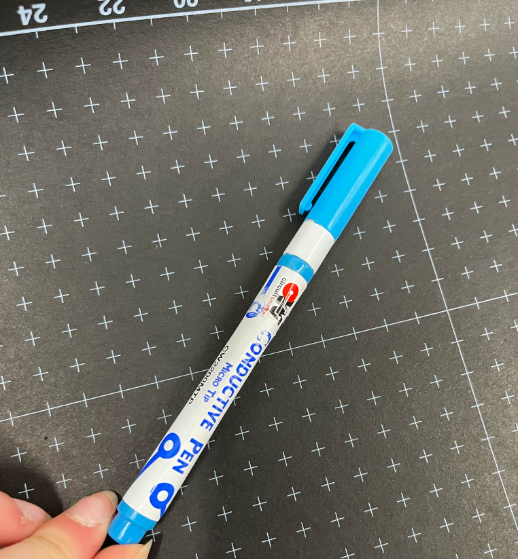
\includegraphics[width=\linewidth]{screenshot002}
		\caption{Paper conductor i retolador de tinta basada en una suspensió de plata.}
		\label{fig1.1a}
	\end{subfigure}
	\hfill
	\begin{subfigure}{0.45\textwidth}
		\centering
		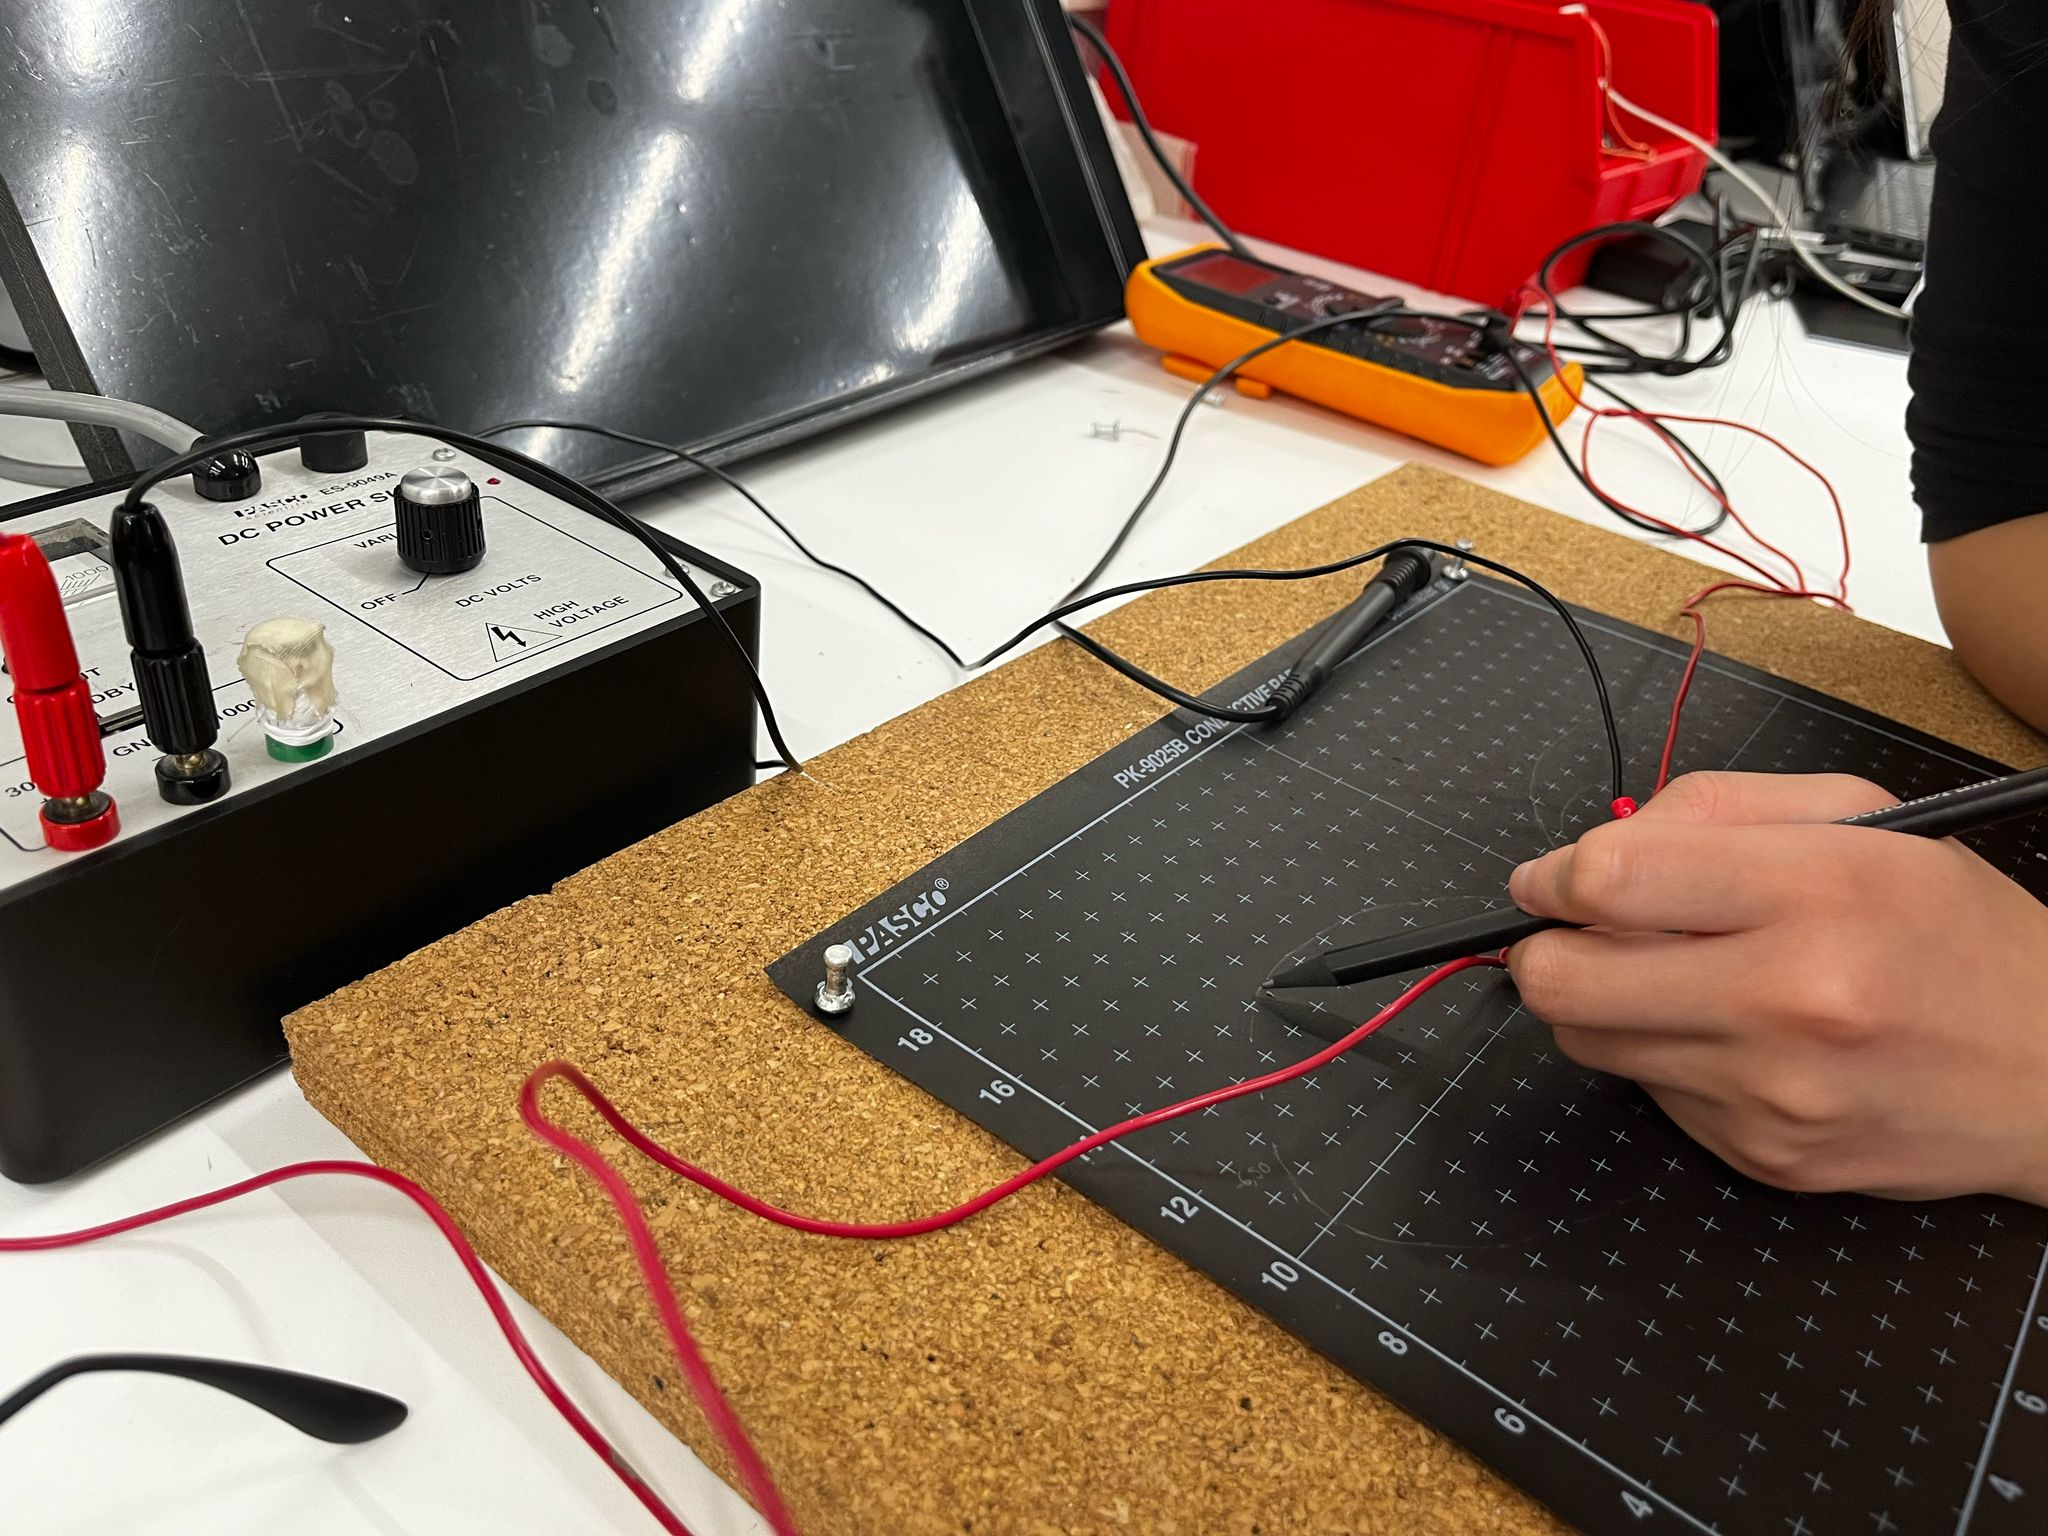
\includegraphics[width=\linewidth]{screenshot003}
		\caption{Muntatge experimental per a la representació de les corbes equipotencials pels dos fils infinits. D'esquerra a dreta: Font de corrent DC connectada als dos elèctrodes (dos punts pel cas representat) mitjançant dos cables; suro amb el paper conductor en el que prèviament s'han dibuixat els dos elèctrodes, enganxat amb xinxetes; multímetre usat per mesurar les diferències de potencial.}
		\label{fig1.1b}
	\end{subfigure}
	\caption{Paper conductor i muntatge experimental per a la representació de les corbes equipotencials.}
	\label{fig1.1}
\end{figure}

Hem treballat amb les següents 3 distribucions: dues línies verticals (que són la projecció d'un condensador de plaques planoparal·leles), dos punts (projecció de dos fils infinits) i dues línies secants amb un punt entre elles (projecció de dos plans infinits formant angle d'aproximadament 60 º amb un fil infinit entre els dos).

Amb el pretext de generar el camp sobre les distribucions dibuixades, s'ha fixat el paper conductor (en el qual hem fet els dibuixos) sobre un suro usant xinxetes i hem connectat els elèctrodes (per a cada distribució per separat) a una font de corrent continu (DC) usant un parell de cables i més xinxetes. Per mesurar la diferència de potencial hem usat un multímetre, deixant un cable fixat a un dels dos elèctrodes (establint així una referència de potencial) i l'altre lliure per tal de fer mesures de $\Delta V$ a qualsevol altre punt del paper (veure figura \ref{fig1.1b}). Prèviament, però, ens hem assegurat què la diferència de potencial entre dos punts en els conductors (els elèctrodes dibuixats) no fos major de l'1\%\footnote{Recordem que, per ser aquests materials conductors, hem de tenir un potencial constant en tot el seu volum i, en particular, sobre la seva superfície.}.

Per dibuixar les corbes equipotencials usem el cable lliure del multímetre per buscar aquestes corbes sobre el paper. Marquem tots els punts que estan a un mateix potencial amb un llapis i, tot seguit, unim aquests punts amb una línia. Repetint això un seguit de cops podem construir vàries corbes equipotencials. Per tal d'assegurar-nos que es tanquen, és millor que comencem a buscar les corbes des de l'exterior dels nostres elèctrodes. Si comencem per l'interior, com que tindrem una densitat de corbes molt major, serà més fàcil que la línia escollida no s'acabi tancant. Veurem que ens interessa trobar corbes que tanquin els nostre elèctrodes per tal de poder aplicar el teorema de Gauss (en especial pel cas del condensador de plaques planoparal·leles).

Finalment, per representar el camp elèctric $\vec{E}$, hem dibuixat línies que sortien dels elèctrodes i tallaven les corbes equipotencials perpendicularment (en ambdós casos). 

\subsection{Càlcul de la capacitat del condensador}
Si aproximem la integral donada per l'equació \eqref{eq1.13} per un sumatori i calculem el camp $E_i$ segons
\begin{equation}
	E_i \approx \frac{\Delta V_i}{\Delta r_i}
\end{equation}
on $\Delta r_i$ és la distància radial i $\Delta V_i$ és la diferència de potencial de l'element $\Delta l_i$ tenim:
\begin{equation}
	\frac{q}{Z} \approx \varepsilon \sum_i \frac{\Delta V_i \Delta l_i}{\Delta r_i}
\end{equation}
Usant que la capacitat d'un condensador de plaques planoparal·leles es correspon amb 
\begin{equation}
	c = \frac{q}{\Delta V}
\end{equation}
tenim que la capacitat per unitat de longitud, sota les aproximacions usades és:
\begin{equation}
	\frac{c}{Z} = \frac{Q/Z}{\Delta V} = \frac{\varepsilon}{\Delta V} \sum_i \frac{\Delta V_i \Delta l_i}{\Delta r_i} \label{eq1.17}
\end{equation}
on $\Delta V$ és la diferència de potencial a la que hem sotmès les dues plaques del condensador.

\subsection{Simulacions}
Els codis de les simulacions es poden trobar a l'annex \ref{an:a4}.

Per la simulació del condensador planoparal·lel, hem considerat la projecció com la contribució de 200 carregues puntuals (totes del mateix valor, pel fil esquerra de valor -q, pel dret q) distribuïdes uniformement a través de cada fil. Un fil es troba a $x = d/2$, i el segon a $x = - d/2$. Les carregues van des de $y = -H/2$ fins $y = H/2$. Per a cada una de les càrregues, hem calculat la seva contribució al camp elèctric i al potencial elèctric en tots els punts de la malla $(X, Y)$, que ho hem fet utilitzant el principi de superposició.

Per a la simulació dels dos fils infinits paral·lels, hem considerat la seva projecció com dues càrregues puntuals separades una distància $(d+2r)$, on aquest valor correspon a la separació entre els centres dels discos dibuixats experimentalment.

Hem definit les funcions que descriuen el potencial i el camp elèctric, que corresponen a les expressions analítiques d'aquests magnituds per a una càrrega puntual. Es calcula la contribució de cada càrrega en tots els punts de la malla i  apliquem el principi de superposició per obtenir el camp elèctric i el potencial total en cada punt de l’espai.

Per la simulació de........

\section{Resultats i discussió}
Els resultats experimentals es poden trobar a l'annex \ref{an:a2}.
\subsection{Condensador de plaques planoparal·leles}
\textbf{S'HA DE FER}
\subsection{Fils infinits}
La segona configuració estudiada és la projecció en el pla $XY$ (pla de la imatge) de dos fils infinits separats per una distància constant. 

Les corbes equipotencials trobades experimentalment són les que es poden observar a la figura \ref{fig:1.2a}. Observem com aquestes formen el·lipses on els fils estan cada cop més descentrats conforme agafem corbes més externes. 
\begin{figure}[h]
	\centering
	\begin{subfigure}{0.45\linewidth}
		\centering
		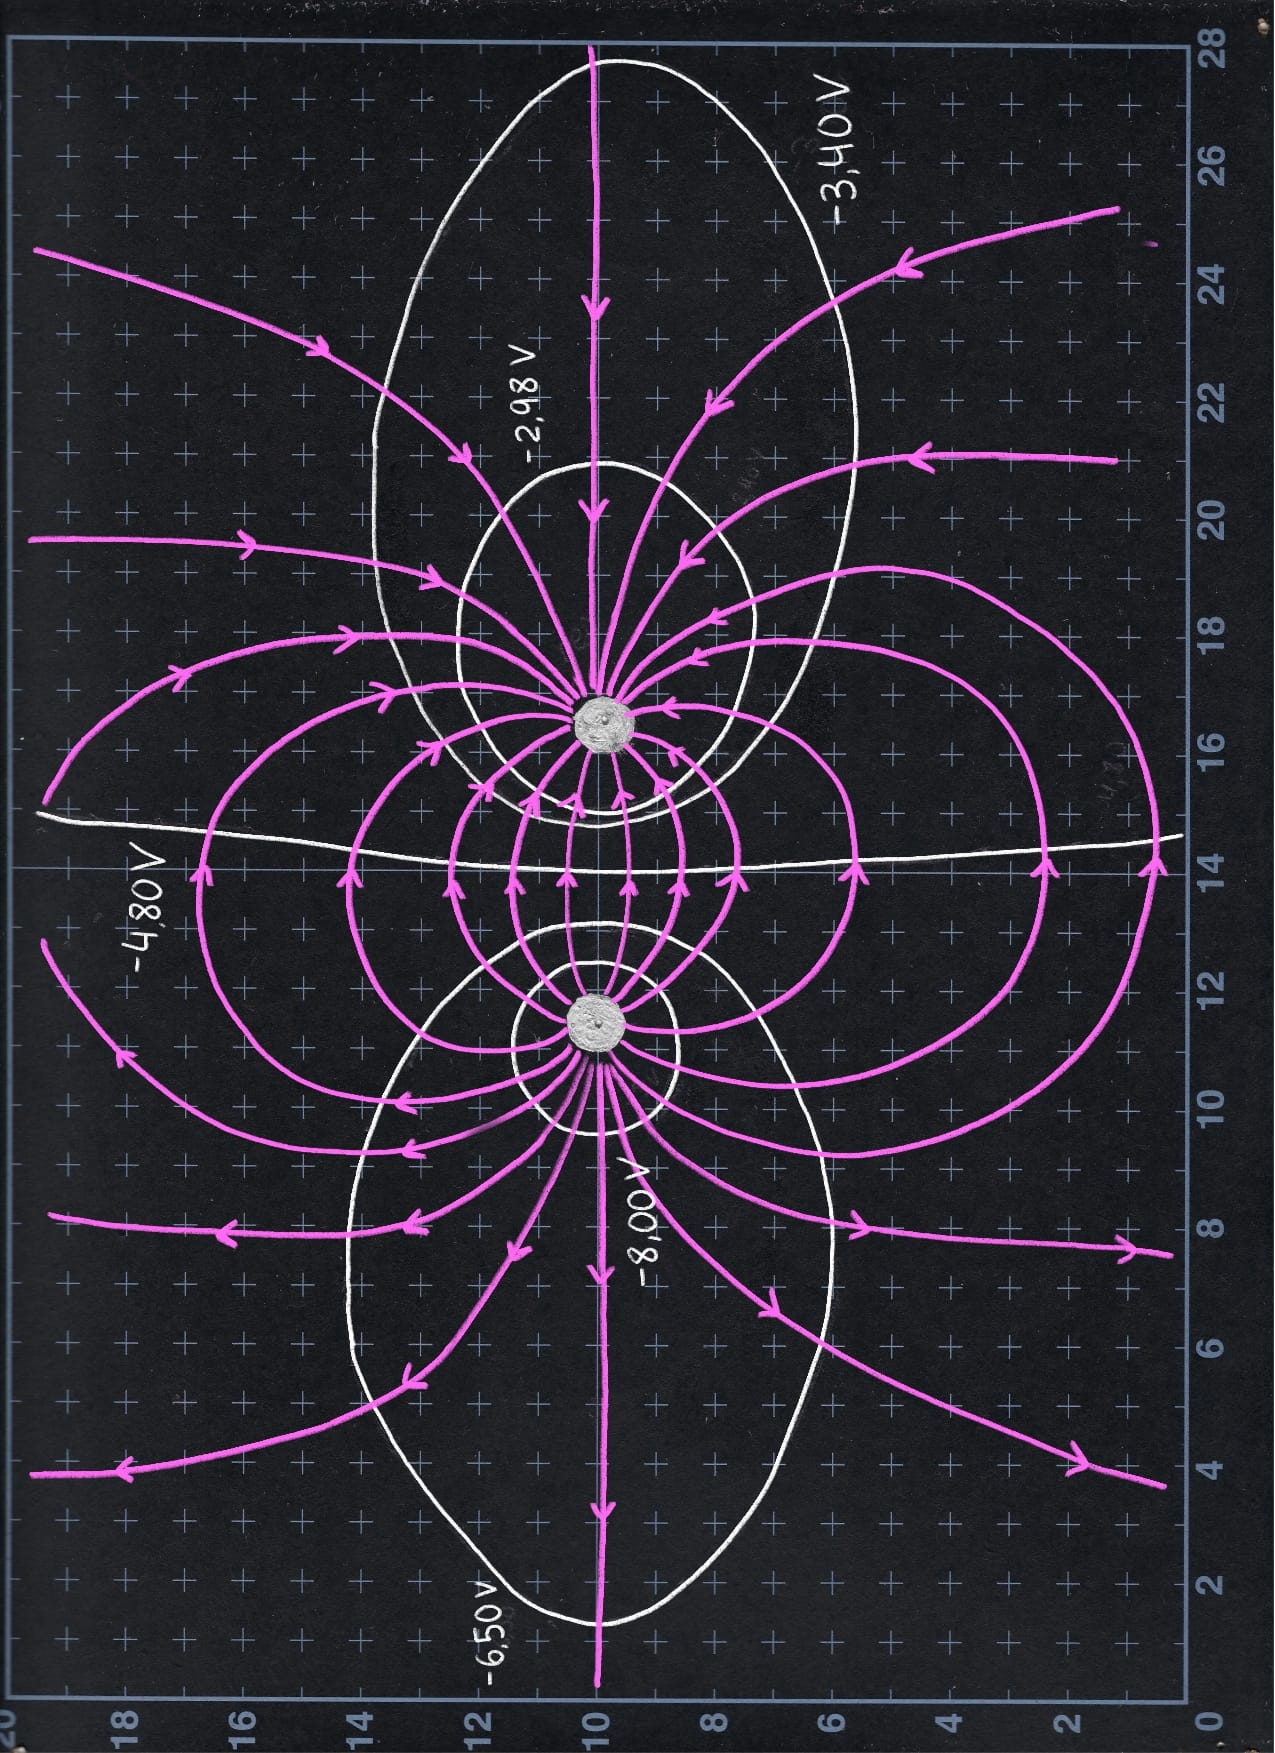
\includegraphics[width=\linewidth]{screenshot004}
		\caption{Corbes equipotencials (en blanc) i línies de camp $\vec{E}$ (en lila) pel cas dels dos fils infinits trobades experimentalment.}
		\label{fig:1.2a}
	\end{subfigure}
	\hfill
	\begin{subfigure}{0.5\linewidth}
		\centering
		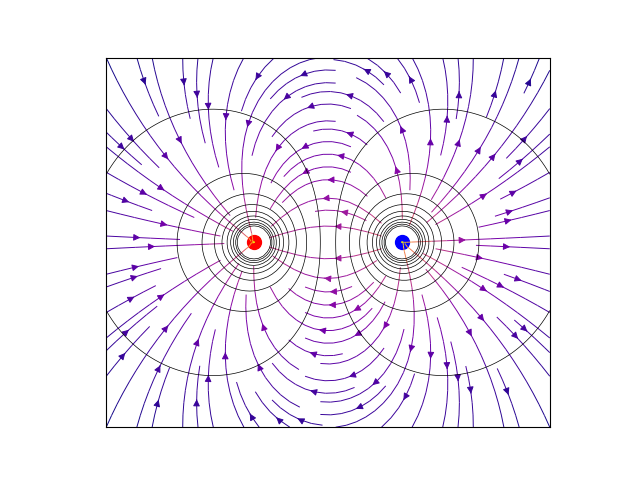
\includegraphics[width=\linewidth]{figfils}
		\caption{Simulació del camp elèctric i del potencial pels dos fils infinits.}
		\label{fig:1.2b}
	\end{subfigure}
	\caption{Representació i simulació de les corbes equipotencials i línies de camp per la distribució de dos fils infinits.}
	\label{fig:1.2}
\end{figure}

Els resultats teòrics indiquen que, en un sistema de dos fils infinits, les corbes equipotencials vénen donades per la següent equació:
\begin{equation}
	y^2+\left( x+a\frac{1+k^2}{1-k^2}\right)^2 = a^2\left( \frac{2k}{1-k^2}\right)^2  \label{eqsuppon}
\end{equation}
Que és l'equació d'una circumferència, de manera que, teòricament, les corbes equipotencials haurien de ser circumferències de radi $R = a\frac{2k}{1-k^2}$ que tenen el seu centre lleugerament desplaçat en l'eix de les $x$ per un factor $a\frac{1+k^2}{1-k^2}$. Notem que tant $a$ com $k$ són dues constants\footnote{Els valors de les constants i la demostració d'aquest resultat es pot trobar a l'annex \ref{an:a1}.}. Es pot veure que això és exactament així si ens atenim als resultats obtinguts a la simulació de la figura \ref{fig:1.2b}.

El fet que els nostres resultats es desviïn del predit per la teoria és degut als diferents errors experimentals comesos durant l'evolució de la pràctica: S'assumeix que el paper conductor té una conductivitat $\sigma$ homogènia, però això no necessàriament ha de ser així (pot ser que presenti inhomogeneïtats), de forma que els resultats de l'experiment es poden veure alterats; els punts que representen la projecció dels dos fils infinits en el pla no són perfectament rodons, ja que han sigut dibuixats a ma (amb les imprecisions que això comporta); les corbes equipotencials i les línies de camp es poden veure afectades per l'efecte punta en les vores dels materials carregats, on s'acumula més densitat de càrrega. 


\subsection{Fil infinit i dos plans}

\textbf{S'HA DE FER}(no oblidar la motivació de la distribució)

\section{Conclusions}
Aquesta pràctica s'ha basat en l'ús d'un multímetre per tal de mesurar el potencial elèctric a diferents distàncies de les distribucions de càrrega dibuixades. Això ens ha permès, per una banda, traçar línies equipotencials i, per altra, obtenir un valor de la capacitat d'un condensador.

Pel que fa a les línies equipotencials, aquestes ens han servit de guia per dibuixar, posteriorment, les respectives línies de camp elèctric, ja que, com ja sabem de teoria, aquestes són perpendiculars a les equipotencials. A més a més, per a les tres geometries considerades, hem generat les corresponents simulacions per tal de poder comparar els resultats experimentals amb els teòrics amb més facilitat.

Tal i com s'ha anat mencionant, el dibuix experimental i la simulació, tot i tenir tendències similars (EXPLICAR LES TENDENCIES BLABLABLALBA)

\chapter{Força entre corrents}
\begin{chapterabstract}
	En aquesta pràctica mesurem la força entre dos fils pels quals hi circula un corrent elèctric, comprovant que la llei de Biot i Savart se satisfà, via diferents metodologies. Amb aquests resultats fem una estimació de la permeabilitat magnètica $\mu_0$, tot comparant-la amb el valor teòric. A més a més, utilitzant el mateix sistema, mesurem la component horitzontal del camp magnètic terrestre al laboratori.
\end{chapterabstract}
\section{Introducció i fonament teòric}
Per quantificar la interacció magnètica entre dos circuits arbitraris tancats pels quals hi circula un corrent constant, és a dir, per mesurar la força que fa un circuit sobre l'altre podem usar que:
\begin{equation}
	\vec{F}_1 = \frac{\mu_0}{4\pi}I_1I_2\oint \oint \frac{\mathrm{d}\vec{l}_1\cross[\mathrm{d}\vec{l}_2 \cross (\vec{r}_1-\vec{r}_2)]}{\abs{\vec{r}_1 - \vec{r}_2}^3}\label{eq:2.1}
\end{equation}
on $\mu_0$, $I_1$ i $I_2$ són les intensitats dels circuits 1 i 2, respectivament, d$\vec{l}_1$ i d$\vec{l}_2$ són els elements infinitesimals de línia i $\vec{r}_1$ i $\vec{r}_2$ són les respectives posicions d'aquests elements.

Per tal de simplificar la integral anterior definim el camp d'inducció magnètica (o densitat de flux magnètic) $\vec{B}(\vec{r})$ en un punt arbitrari $\vec{r}$ com:
\begin{equation}
	\vec{B}(\vec{r}) = \frac{\mu_0}{4\pi} \int_V \vec{J}(\vec{r}_1)\cross\frac{\vec{r}-\vec{r}'}{\abs{\vec{r}-\vec{r}'}^3}\mathrm{d}^3r'
\end{equation} 
Si usem això sobre l'equació \eqref{eq:2.1} podem escriure la força que rep el circuit amb intensitat I degut a la presència del camp d'inducció $\vec{B}$ creat per l'altre circuit segons:
\begin{equation}
	\vec{F} = I \oint \mathrm{d}\vec{l}\cross\vec{B}(\vec{r})
\end{equation}
Emprant una de les equacions pel camp $\vec{B}$
\begin{equation}
	\vec{\nabla}\cross \vec{B} = \mu_0 \vec{J}
\end{equation}
i aplicant el teorema de Stokes
\begin{equation}
	\oint_C \vec{A} \cdot \mathrm{d}\vec{r} = \int_S (\vec{\nabla}\cross \vec{A})\cdot \mathrm{d}\vec{S}
\end{equation}
podem deduir fàcilment el teorema d'Ampère, que ens diu que:
\begin{equation}
	\oint_C\vec{B}\cdot\mathrm{d}\vec{l} = \mu_0\int_S\vec{J}(\vec{r})\cdot\vec{n}\mathrm{d}S
\end{equation}
d'on, mitjançant un càlcul ràpid podem trobar el camp d'inducció magnètica generat per un fil infinit amb intensitat $I$ a una distància $r$ del seu centre:
\begin{equation}
	B = \frac{\mu_0 I}{2\pi r}
\end{equation}
Així doncs, la força, en mòdul que patirà un altre fil (infinit) paral·lel, de longitud $L$ i que és perpendicular al camp $\vec{B}$ serà:
\begin{equation}
	F = \frac{\mu_0 I^2L}{2\pi r}
\end{equation} 
\section{Metodologia experimental}

\subsection{Equilibrat de la balança}
\subsection{Força vs. corrent}
\subsection{Força vs. separació}
\subsection{Mesura del camp magnètic terrestre}

\section{Resultats i discussió}

\subsection{Valor experimental de la permeabilitat magnètica}
\subsection{Camp magnètic terrestre}

\section{Conclusions}

\begin{thebibliography}{99}
	\bibitem{ref1}
	\textit{Col·lecció de problemes de l'assignatura d'Electromagnetisme.}
\end{thebibliography}




\newpage
\begin{appendices}
%SI TOQUEU AIXÒ ELS ANNEXOS PETEN.

\textbf{\Huge{Annexos}}
\renewcommand{\thesection}{\Alph{section}} % Cambia la numeración de capítulos a letras
\renewcommand{\theequation}{\thesection.\arabic{equation}} % Cambia numeración de ecuaciones
\setcounter{equation}{0} % Reinicia contador de ecuaciones en cada sección
\section{Pràctica 1. Representació de camps}
\subsection{Deducció de l'equació \eqref{eqsuppon}}
\label{an:a1}
Per deduir l'expressió donada per l'equació \eqref{eqsuppon} ens basarem ens els resultats del problema 2.18 de la llista de problemes de l'assignatura \cite{ref1}. Suposem dos fils infinits rectilinis i carregats amb densitat de càrrega uniforme $\lambda$ i -$\lambda$ separats per una distància $d=2a$. Siguin $\rho_1$ i $\rho_2$ les distàncies radials de cada fil al punt en el qual volem calcular el camp i el potencial. Per la simetria del sistema podem assegurar que $\vec{E}(\vec{r}) = E(\rho) \vec{e}_{\rho}$, de forma que podem aplicar el teorema de Gauss com se segueix:

\[
\left.
\begin{array}{c}
	\oint \vec{E} \cdot \mathrm{d}\vec{S} = E 2\pi \rho L \\[10pt]
	\frac{Q_{int}}{\varepsilon_0} = \frac{1}{\varepsilon_0} \int \lambda \, \mathrm{d}l = \frac{\lambda}{\varepsilon_0} L
\end{array}
\right\}
\quad \Rightarrow \quad 
\vec{E} = \frac{\lambda}{2\pi \varepsilon_0} \frac{1}{\rho} \vec{e}_{\rho}
\]

Així, essent $\vec{E_1}$ el camp associat al fil amb densitat $\lambda$ i $\vec{E_2}$ el camp associat al fil amb densitat -$\lambda$, tenim:
\begin{align}
	\vec{E_1} & = \frac{\lambda}{2\pi \varepsilon_0} \frac{1}{\rho_1} \vec{e}_{\rho_1} \\
	\vec{E_2} & = -\frac{\lambda}{2\pi \varepsilon_0} \frac{1}{\rho_2} \hat{e}_{\rho_2}
\end{align}
on:
\begin{align}
	\rho_1 & = \sqrt{(x-a)^2+y^2} \\
	\rho_2 & = \sqrt{(x+a)^2+y^2} 
\end{align}

Si calculem el camp usant que
\begin{equation}
	\phi(r) = -\int_{\vec{r}_{ref}}^{\vec{r}}\vec{E}(\vec{r})\cdot \mathrm{d}\vec{r} 
\end{equation}
i aplicant el principi de superposició, és a dir
\begin{equation}
	\phi = \phi_1+\phi_2
\end{equation}
trobem que, el potencial generat per aquesta distribució de càrrega obeeix la següent equació:
\begin{equation}
	\phi = \frac{\lambda}{2\pi \varepsilon_0}\ln\sqrt{\frac{(x+a)^2+y^2}{(x-a)^2+y^2}}
\end{equation}
Escollint
\begin{equation}
	k \equiv e^{\frac{\phi2\pi\varepsilon_0}{\lambda}} = \sqrt{\frac{(x+a)^2+y^2}{(x-a)^2+y^2}}
\end{equation}
i reescrivint segons
\begin{equation}
	k^2[(x-a)^2+y^2]=(x+a)^2+y^2
\end{equation}  
podem desenvolupar fins a arribar a
\begin{equation}
	\boxed{y^2+\left( x+a\frac{1+k^2}{1-k^2}\right)^2 = a^2\left( \frac{2k}{1-k^2}\right)^2}
\end{equation}
que és el que estàvem buscant.

\newpage
\subsection{Dades experimentals de la pràctica 1}
\label{an:a2}
A continuació mostrem els valors experimentals obtinguts en el transcurs de la pràctica 1.
\begin{table}[h]
	\centering
	\renewcommand{\arraystretch}{1.2}
	\caption{Taula amb els valors experimentals mesurats per tal de poder calcular la capacitat del condensador de plaques planoparal·leles.}
	\begin{tabular}{cccc}
		\toprule
		$\Delta l_i$ (m) & $\Delta r_i$ (m) & $\Delta V_i$ (V) & $\frac{\Delta V_i\Delta l_i}{\Delta r_i}$ (V)\\
		\midrule
		0.005 $\pm$ 0.001 & 0.019 $\pm$ 0.001 & 1.00 $\pm$ 0.01 & 0.26 $\pm$ 0.23 \\
		0.005 $\pm$ 0.001 & 0.024 $\pm$ 0.001 & 1.00 $\pm$ 0.01 & 0.21 $\pm$ 0.20 \\
		0.010 $\pm$ 0.001 & 0.038 $\pm$ 0.001 & 1.00 $\pm$ 0.01 & 0.26 $\pm$ 0.16 \\
		0.010 $\pm$ 0.001 & 0.050 $\pm$ 0.001 & 1.00 $\pm$ 0.01 & 0.20 $\pm$ 0.14 \\
		0.005 $\pm$ 0.001 & 0.057 $\pm$ 0.001 & 1.00 $\pm$ 0.01 & 0.09 $\pm$ 0.13 \\
		0.005 $\pm$ 0.001 & 0.063 $\pm$ 0.001 & 1.00 $\pm$ 0.01 & 0.08 $\pm$ 0.13 \\
		0.010 $\pm$ 0.001 & 0.070 $\pm$ 0.001 & 1.00 $\pm$ 0.01 & 0.14 $\pm$ 0.12 \\
		0.005 $\pm$ 0.001 & 0.071 $\pm$ 0.001 & 1.00 $\pm$ 0.01 & 0.07 $\pm$ 0.12 \\
		0.009 $\pm$ 0.001 & 0.066 $\pm$ 0.001 & 1.00 $\pm$ 0.01 & 0.14 $\pm$ 0.12 \\
		0.010 $\pm$ 0.001 & 0.034 $\pm$ 0.001 & 1.00 $\pm$ 0.01 & 0.29 $\pm$ 0.17 \\
		0.008 $\pm$ 0.001 & 0.024 $\pm$ 0.001 & 1.00 $\pm$ 0.01 & 0.33 $\pm$ 0.20 \\
		0.005 $\pm$ 0.001 & 0.014 $\pm$ 0.001 & 1.00 $\pm$ 0.01 & 0.36 $\pm$ 0.27 \\
		0.005 $\pm$ 0.001 & 0.009 $\pm$ 0.001 & 1.00 $\pm$ 0.01 & 0.56 $\pm$ 0.34 \\
		0.002 $\pm$ 0.001 & 0.004 $\pm$ 0.001 & 1.00 $\pm$ 0.01 & 0.50 $\pm$ 0.52 \\
		0.002 $\pm$ 0.001 & 0.003 $\pm$ 0.001 & 1.00 $\pm$ 0.01 & 0.67 $\pm$ 0.62 \\
		0.003 $\pm$ 0.001 & 0.004 $\pm$ 0.001 & 1.00 $\pm$ 0.01 & 0.75 $\pm$ 0.53 \\
		0.010 $\pm$ 0.001 & 0.005 $\pm$ 0.001 & 1.00 $\pm$ 0.01 & 2.00 $\pm$ 0.60 \\
		0.010 $\pm$ 0.001 & 0.006 $\pm$ 0.001 & 1.00 $\pm$ 0.01 & 1.67 $\pm$ 0.49 \\
		0.010 $\pm$ 0.001 & 0.006 $\pm$ 0.001 & 1.00 $\pm$ 0.01 & 1.67 $\pm$ 0.49 \\
		0.010 $\pm$ 0.001 & 0.006 $\pm$ 0.001 & 1.00 $\pm$ 0.01 & 1.67 $\pm$ 0.49 \\
		0.010 $\pm$ 0.001 & 0.005 $\pm$ 0.001 & 1.00 $\pm$ 0.01 & 2.00 $\pm$ 0.60 \\
		0.010 $\pm$ 0.001 & 0.005 $\pm$ 0.001 & 1.00 $\pm$ 0.01 & 2.00 $\pm$ 0.60 \\
		0.010 $\pm$ 0.001 & 0.006 $\pm$ 0.001 & 1.00 $\pm$ 0.01 & 1.67 $\pm$ 0.49 \\
		0.005 $\pm$ 0.001 & 0.005 $\pm$ 0.001 & 1.00 $\pm$ 0.01 & 1.00 $\pm$ 0.49 \\
		0.002 $\pm$ 0.001 & 0.005 $\pm$ 0.001 & 1.00 $\pm$ 0.01 & 0.40 $\pm$ 0.45 \\
		0.002 $\pm$ 0.001 & 0.006 $\pm$ 0.001 & 1.00 $\pm$ 0.01 & 0.33 $\pm$ 0.41 \\
		0.003 $\pm$ 0.001 & 0.007 $\pm$ 0.001 & 1.00 $\pm$ 0.01 & 0.43 $\pm$ 0.38 \\
		0.005 $\pm$ 0.001 & 0.011 $\pm$ 0.001 & 1.00 $\pm$ 0.01 & 0.45 $\pm$ 0.30 \\
		\bottomrule
	\end{tabular}
	\label{tab:valores}
\end{table}

Amb aquests valors i usant l'equació \eqref{eq1.17} podem determinar la capacitat del condensador de plaques planoparal·leles dibuixat.

\newpage
\subsection{Càlcul d'incerteses de la pràctica 1}
\label{an:a3}

\newpage
\subsection{Codis de les simulacions de la pràctica 1}
\label{an:a4}
Tot seguit adjuntem els diferents codis usats per generar les simulacions dels camps i les corbes equipotencials usant Python:.

El codi per la simulació del condensador de plaques planoparal·leles és:
\begin{lstlisting}
import numpy as np
import matplotlib.pyplot as plt

# Definim el camp electric 
def E(q, r0, x, y):
rx, ry = x - r0[0], y - r0[1]
dist = (rx**2 + ry**2)**1.5
return q * rx / dist, q * ry / dist

# Definim el potencial electric
def V(q, r0, x, y):
return q / np.hypot(x - r0[0], y - r0[1])

# Malla
x = np.linspace(-6, 6, 100)
y = np.linspace(-5, 5, 100)
X, Y = np.meshgrid(x, y)

q1, q2 = 1, -1
d = 4
charges = [(q1, (d/2, 0)), (q2, (-d/2, 0))]

Ex, Ey = np.zeros(X.shape), np.zeros(Y.shape)
Vt = np.zeros(X.shape)
for q, pos in charges:
ex, ey = E(q, pos, X, Y)
Ex += ex
Ey += ey
Vt += V(q, pos, X, Y)

fig, ax = plt.subplots()
ax.streamplot(X, Y, Ex, Ey, color=np.log(np.hypot(Ex, Ey)), linewidth=0.7, cmap=plt.cm.plasma, density=1)
ax.contour(X, Y, Vt, levels=np.linspace(-2, 2, 20), colors='black', linestyles='solid', linewidths=0.5)

for q, pos in charges:
color = 'red' if q < 0 else 'blue'
ax.scatter(*pos, color=color, s=100)

ax.set_aspect('equal')
ax.set_xticks([])
ax.set_yticks([])
ax.spines['top'].set_visible(True)
ax.spines['right'].set_visible(True)
ax.spines['left'].set_visible(True)
ax.spines['bottom'].set_visible(True)
plt.show()
\end{lstlisting}

El codi per la simulació dels dos fils infinits és:
\begin{lstlisting}
import numpy as np
import matplotlib.pyplot as plt

# Definim el camp electric
def E(q, r0, x, y):
    rx, ry = x - r0[0], y - r0[1]
    dist = (rx**2 + ry**2)**1.5
    return q * rx / dist, q * ry / dist

# Definim el potencial electric
def V(q, r0, x, y):
    return q / np.hypot(x - r0[0], y - r0[1])

# Malla
x = np.linspace(-6, 6, 100)
y = np.linspace(-5, 5, 100)
X, Y = np.meshgrid(x, y)

q1, q2 = 1, -1
d = 4
charges = [(q1, (d/2, 0)), (q2, (-d/2, 0))]

Ex, Ey = np.zeros(X.shape), np.zeros(Y.shape)
Vt = np.zeros(X.shape)
for q, pos in charges:
    ex, ey = E(q, pos, X, Y)
    Ex += ex
    Ey += ey
    Vt += V(q, pos, X, Y)

fig, ax = plt.subplots()
ax.streamplot(X, Y, Ex, Ey, color=np.log(np.hypot(Ex, Ey)), linewidth=0.7, cmap=plt.cm.plasma, density=1)
ax.contour(X, Y, Vt, levels=np.linspace(-2, 2, 20), colors='black', linestyles='solid', linewidths=0.5)

for q, pos in charges:
    color = 'red' if q < 0 else 'blue'
    ax.scatter(*pos, color=color, s=100)

ax.set_aspect('equal')
ax.set_xticks([])
ax.set_yticks([])
ax.spines['top'].set_visible(True)
ax.spines['right'].set_visible(True)
ax.spines['left'].set_visible(True)
ax.spines['bottom'].set_visible(True)
plt.show()
\end{lstlisting}

El codi per la simulació dels dos plans secants i el fil infinit és:
\end{appendices}


\end{document}
